\chapter{Benutzeroberfläche}
\label{ch:benutzeroberfläche}

\begin{figure}
	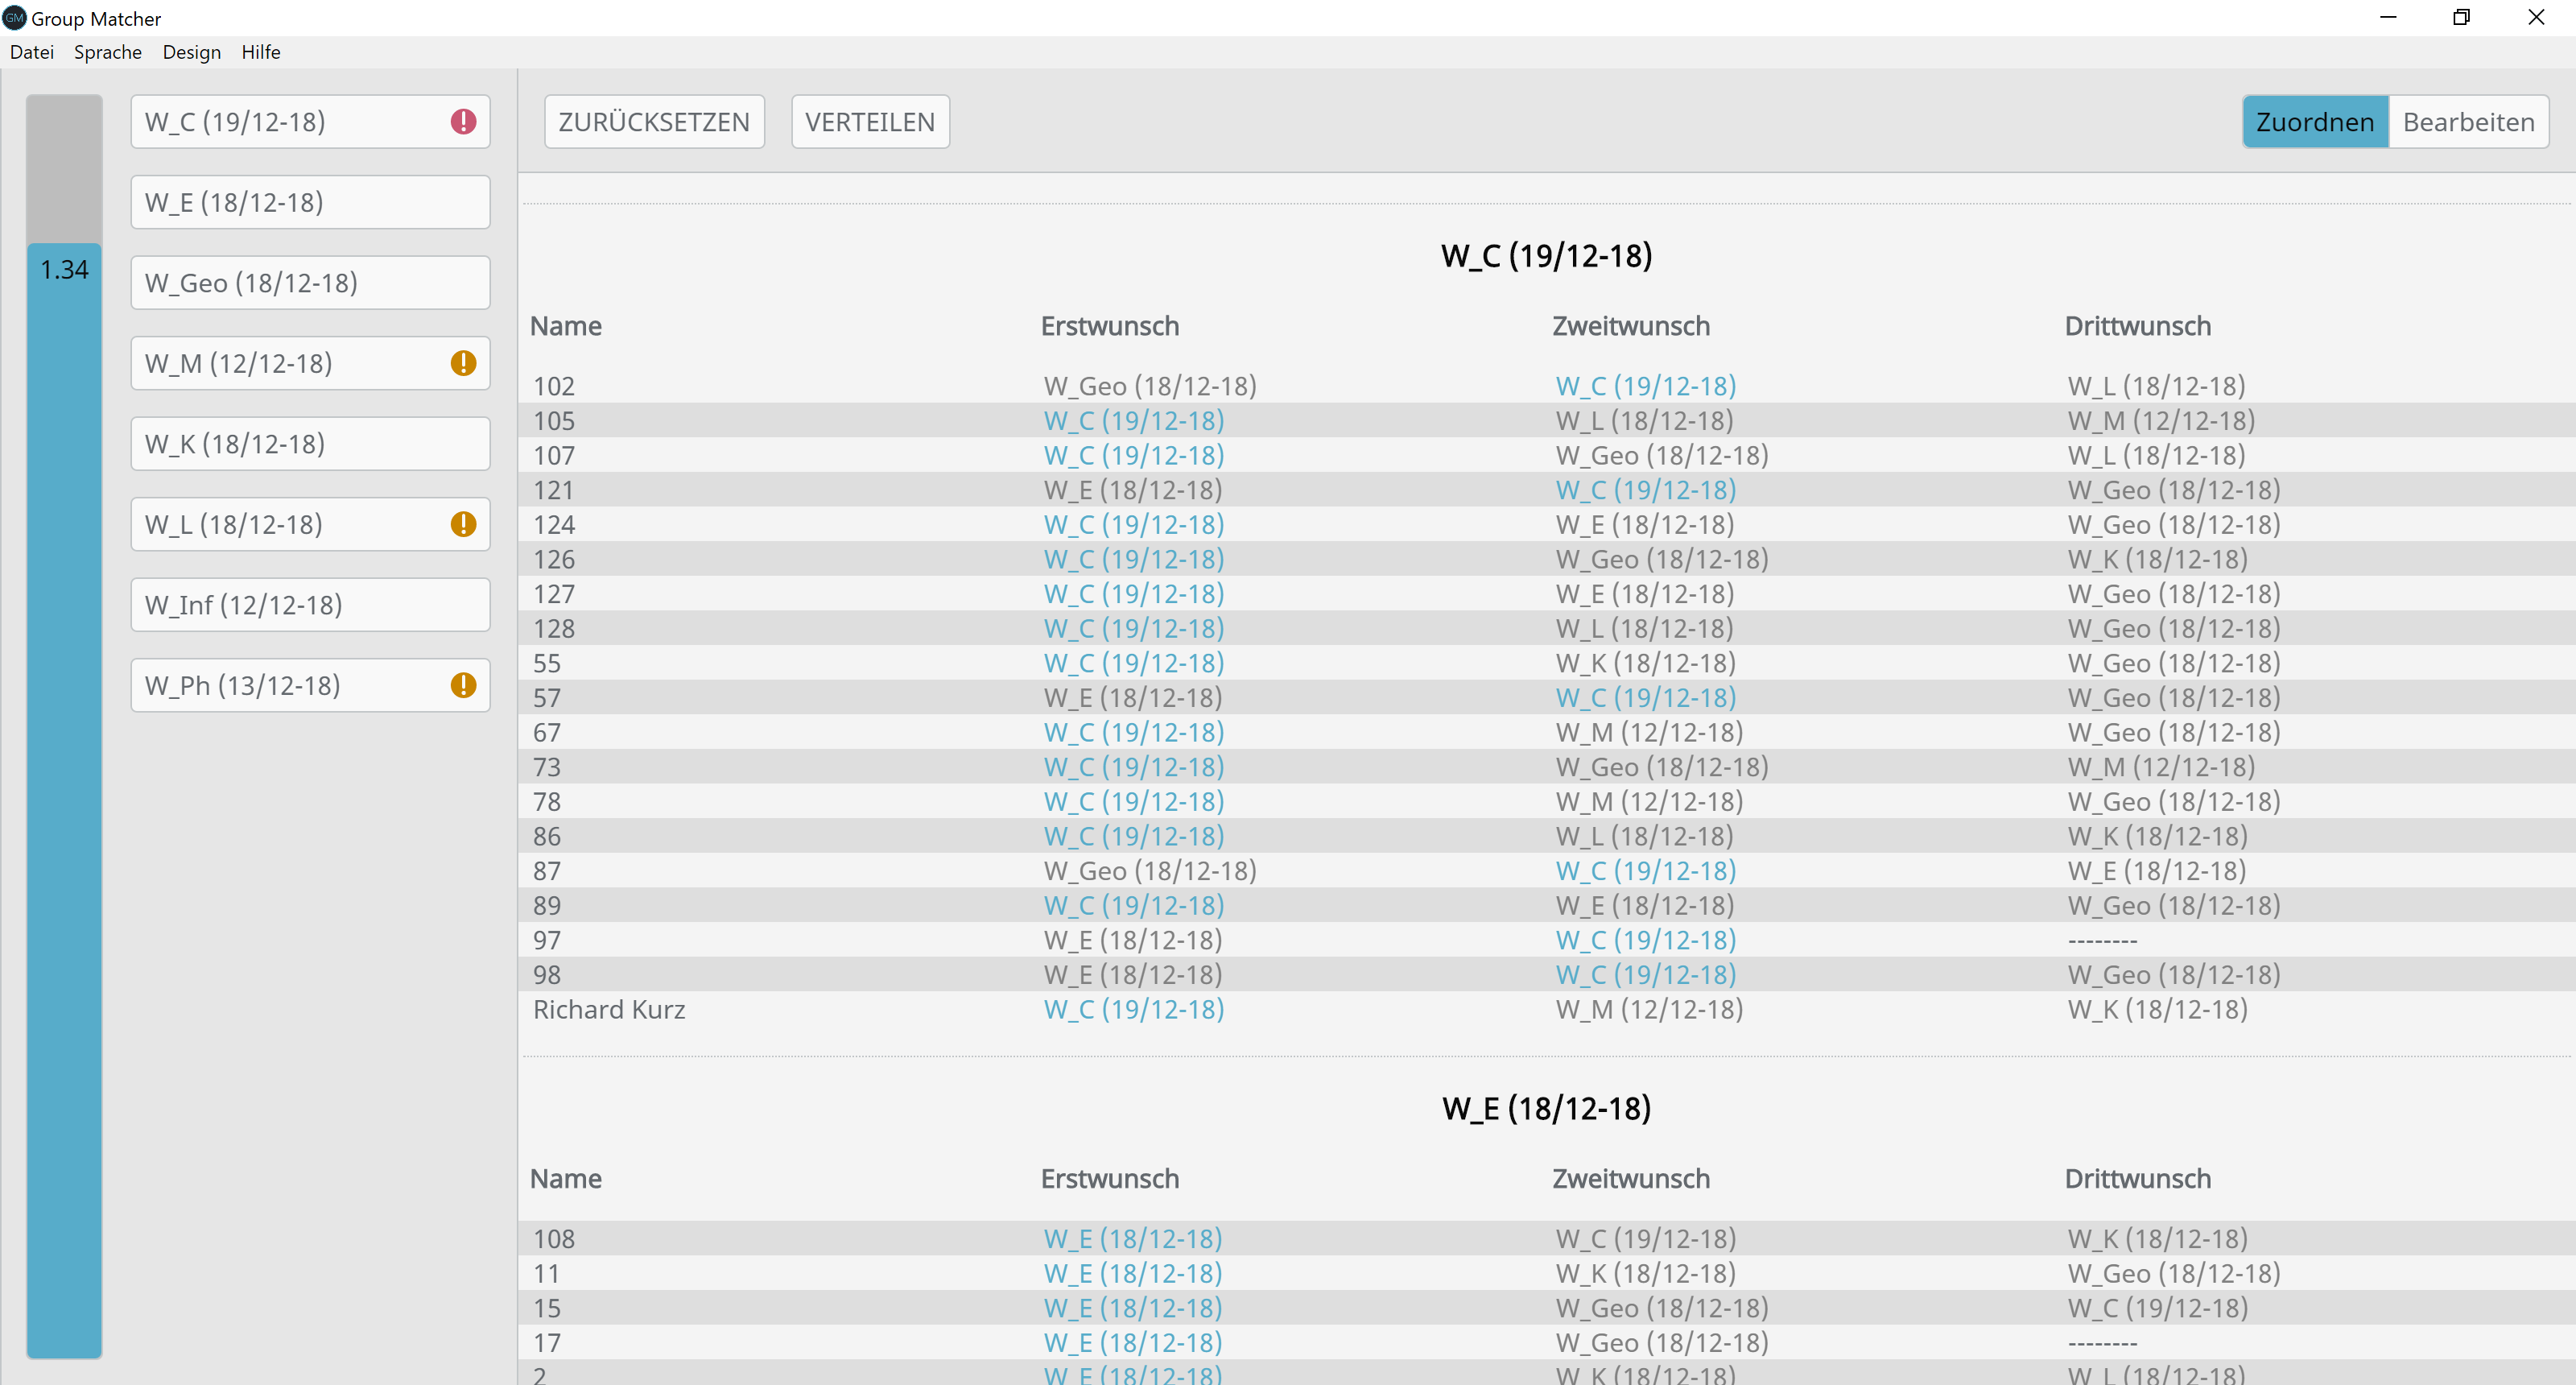
\includegraphics{zuordnungsmodus}
	\caption{Die Benutzeroberfläche}
	\label{fig:die_benutzeroberfläche}
\end{figure}

Die Benutzeroberfläche, die in Abbildung \ref{fig:die_benutzeroberfläche} dargestellt ist, besteht neben \hl{Fehlermeldungen} und \hl{Benachrichtigungen} aus vier Bereichen:
\begin{itemize}
	\item Die \hl{Menüleiste} (\ref{sec:menüleiste}) befindet sich in voller Breite ganz oben im Fenster.
	\item Die \hl{Seitenleiste} (\ref{sec:seitenleiste}) nimmt den linken Rand des Bildschirms ein.
	\item Die \hl{Bedienzeile} (\ref{sec:bedienzeile}) ist links von der Seitenleiste und oben von der Menüleiste begrenzt.
	\item Die \hl{Arbeitsfläche} (\ref{sec:arbeitsfläche}) nimmt den Rest des Fensters ein.
\end{itemize}
Während die Menüleiste und die Seitenleiste stets unverändert bleiben, ist der Inhalt von Bedienzeile und Arbeitsfläche abhängig vom aktuellen Programmmodus. Dabei gibt es auf der einen Seite den \hl{Zuordnungsmodus}, der es ermöglicht, wie der Name schon sagt, die Personen den Gruppen zuzuordnen. Auf der anderen Seite gibt es noch den \hl{Bearbeitungsmodus}, in dem die >>.gm<< Datei des Projekts bearbeitet werden kann. Hier erstellt oder bearbeitet man also ein Projekt, indem man in der in Abschnitt \ref{sec:>>.gm<<_syntax} beschriebenen Syntax Gruppen und Personen erstellt.\\
Im Folgenden werden die vier Bedienelemente der Oberfläche genauer erklärt.

\section{Menüleiste}
\label{sec:menüleiste}

Die Menüleiste dient zur Kontrolle von Programm und Projekt. Sie enthält vier Unterpunkte.

\paragraph{Datei} Hier ist zunächst die Kontrolle des Projekts, also der >>.gm<< Datei \mnote{Im Dateiformat >>.gm<< speichert der >>GroupMatcher<< zum einen die Projekte ab. Zum anderen dient das Format auch zur schnellen Erstellung eines Projekts. Die Syntax dafür wird in Kapitel \ref{ch:erstellen_eines_projekts} beschrieben.} möglich.
\begin{itemize}
	\item \hl{Öffnen...} (öffnet einen Dialog, der das einlesen eines Projekts, also einer >>.gm<< Datei ermöglicht)
	\item \hl{Schließen} (schließt das Projekt, ohne den aktuellen Zustand zu speichern)
	\item \hl{Speichern} (speichert den aktuellen Stand in die geöffnete >>.gm<< Datei)
	\item \hl{Speichern unter...} (öffnet einen Dialog, der das Speichern des aktuellen Standes in eine neue >>.gm<< Datei ermöglicht, und schließt (sofern vorhanden) die alte >>.gm<< Datei)
	\item \hl{Exportieren...} (öffnet einen Dialog, der das erstellen einer Excel-Datei, welche das Projekt darstellt, ermöglicht)
	\paragraph{Excel (begrenzt)} Die begrenzte Version enthält lediglich die Liste der Personen in alphabetischer Reihenfolge mit dem jeweils zugeordneten Wunsch.
	\paragraph{Excel (komplett)} Die komplette Version gibt alle Projektinformationen wieder. Sie listet alle Gruppen mit minimaler und maximaler Mitgliederzahl, sowie der nach der Zuteilung tatsächlich entstandenen Gruppenstärke auf. Zudem stellt sie jede Person mit ihren Wünschen dar und hebt dabei den ihr zugeteilten farblich hervor.
	\item \hl{Beenden} (schließt das Programm und speichert, insofern schon eine >>.gm<< Datei erstellt wurde, das Projekt in diese ab)
\end{itemize}

\paragraph{Sprache} Dieses Untermenü ermöglicht das Wechseln zwischen den bereitgestellten Sprachen.

\paragraph{Design} Neben den hellen Standarddesign lässt sich bei dunkler Umgebung auf das für die Augen angenehmere dunkle Design umschalten.

\paragraph{Hilfe} Neben dem öffnen dieser Dokumentation im Punkt >>Hilfe<< können hier im Punkt >>Über GroupMatcher<< weitere Informationen über Ursprung, aktuelle Versionen und Lizensierung des Programms gewonnen werden.

\section{Seitenleiste}
\label{sec:seitenleiste}

Die Seitenleiste gibt eine Übersicht über das Projekt und erleichtert die Navigation in der Arbeitsfläche. Die blaue Skala zeigt die aktuelle Quote \mnote{Die Quote gibt an, wie zufrieden die Personen durchschnittlich mit ihrer Zuteilung sind. Die Berechnung wird in Abschnitt \ref{sec:verteilungsalgorithmus} genauer erläutert. Generell gilt aber, je höher der blaue Balken, desto besser das Ergebnis.}.\\
Rechts daneben sind alle Gruppen aufgelistet. Dabei wird erst der Gruppenname und dann in Klammern zunächst die aktuelle Gruppenstärke, dann die Mindest- und Maximalgröße der Gruppe angezeigt. Drückt man auf den Knopf einer Gruppe, so scrollt die Arbeitsfläche zu deren Position. Die Knöpfe können zwei verschiedene Warnungen anzeigen. Erscheint ein orangenes Ausrufezeichen, dann bedeutet dies, dass die Gruppe ein Mitglied hat, das unzufrieden \mnote{Unzufriedenheit bedeutet dabei, dass der Person ein Wunsch zugeordnet wurde, der in der hinteren Hälfte seiner Wunschliste steht.} mit seiner Zuteilung ist. Leuchtet stattdessen ein rotes Ausrufezeichen auf, so widerspricht die aktuelle Gruppenstärke der Mindest- oder Maximalgröße der Gruppe. Dieser Fall tritt jedoch nie durch die automatische Verteilung auf, sondern kann nur in der manuellen Nachverteilung herbeigeführt werden. Mehr zum Verteilungsvorgang finden sie in Kapitel \ref{ch:verteilen_der_personen}.

\section{Bedienzeile}
\label{sec:bedienzeile}

Hier sind Knöpfe mit Aktionen zum verändern des Projekts sowie einem Wechselschalter angebracht. Letzterer ermöglicht das Umschalten zwischen den verschiedenen Programmmodi.
\paragraph{Aktionen} Im Zuordnungsmodus sind die Aktionen >>Zurücksetzen<< und >>Verteilen<< verfügbar. Dabei hebt erstere sämtliche Zuordnungen auf während zweitere den automatischen Verteilungsalgorithmus \mnote{Der Verteilungsalgorithmus stellt den Kern des Programmes dar. Er verteilt in Bruchteilen einer Sekunde die Personen unter Beachtung aller gegebenen Vorschriften auf die Gruppen. Genaueres zu dessen Prioritäten und Anwendung finden sie in Kapitel \ref{ch:verteilen_der_personen}.} startet. Im Bearbeitungsmodus hingegen sind keine Aktionen verfügbar.
\paragraph{Wechselschalter} Der Wechselschalter befindet sich am rechten Rand der Bedienzeile und ermöglicht das Wechseln zwischen Bearbeitungs- und Zuordnungsmodus. Dabei ist der aktuell ausgewählte Modus blau hinterlegt. Befindet man sich im Bearbeitungsmodus werden beim Betätigen des Schalters neben dem Wechseln zum Zuordnungsmodus automatisch die vorgenommenen Änderungen an der >>.gm<< Datei ausgewertet. Wird dabei ein Fehler erkannt, wird dieser angezeigt und im Textfeld \mnote{Das Textfeld befindet sich im Bearbeitungsmodus in der Arbeitsfläche.} die betroffene Zeile rot markiert. Das wechseln zum Zuordnungsmodus wird also in Bearbeitungsmodus solange verweigert, bis die >>.gm<< Datei keinen Fehler mehr enthält und übersetzt werden kann.

\section{Arbeitsfläche}
\label{sec:arbeitsfläche}

Die Arbeitsfläche nimmt den Großteil des Fensters ein und stellt auch die meisten Informationen dar. Dabei muss wieder zwischen den Programmmodi differenziert werden.
\paragraph{Zuordnungsmodus} Hier enthält die Arbeitsfläche eine Tabelle mit allen Gruppen und Personen. Unter jeder Gruppenüberschrift sind die ihr zugeordneten Personen \mnote{Unzugeordnete Personen haben eine eigenen Gruppe namens >>Unzugeordnet<<.} aufgelistet. In der ersten Spalte steht dabei der Name der Person, in der zweiten der Erstwunsch, in der dritten der Zweitwunsch und in der vierten der Drittwunsch. Bei den wünschen ist neben dem Namen der gewünschten Gruppe auch die aktuelle Größe sowie Minimal- und Maximalgröße angegeben. Dies führt zu äußerst hoher Effektivität bei manueller Nachverteilung, denn klickt man auf einen Wunsch, so wird die Person in diesen Wunsch verschoben. Dem ist nicht so, wenn der Wunsch blau markiert ist, da dieser Wunsch der Erfüllte ist, er stellt also die Gruppe dar, in der sich die Person aktuell befindet. In diesem Fall wird die Person wieder unzugeordnet.
\paragraph{Bearbeitungsmodus} In diesem Zustand enthält die Arbeitsfläche nicht die Tabelle, sondern lediglich ein großes Textfeld. Darin wird die >>.gm<< Datei des Projekts angezeigt bzw. hier können sie diese erstellen. Das Textfeld ist links mit Zeilenzahlen versehen, was das Finden eines Fehlers im Code erheblich erleichtert \mbox{Die betroffene Zeile wird rot markiert.}.

\section{Mitteilungen}
\label{sec:mitteilungen}

Wenn das Programm Mitteilungen für sie hat geschieht dies in Form eines rechteckigen Feldes im oberen rechten Eck der Arbeitsfläche. Ist es eine \hl{Benachrichtigung} \mnote{Benachrichtigungen verschwinden nach einigen Sekunden von alleine.}, so ist sie blau hinterlegt und dient nur zur Bestätigung eines Vorgangs. Trat jedoch ein \hl{Fehler} auf, so ist die Mitteilung \mnote{Stört die Fehlermeldung die Sicht, so kann sie per Mausklick entfernt werden.} rot hinterlegt. Die Bedeutung sämtlicher Fehlermeldungen finden sie im Kapitel \ref{ch:fehlermeldungen}.
